\documentclass[rgb]{beamer}

\usepackage[english]{babel}
\usepackage[utf8]{inputenc}
\usepackage{xcolor}
\usepackage{listings}
\usepackage{adjustbox}
\usepackage{amsmath}
\usepackage{multirow}
\usepackage[linewidth=1pt]{mdframed}

% Graphics
\usepackage{graphicx}

\usepackage{tikz}
\usetikzlibrary{calc,shapes.multipart,chains,arrows}

% Font
\usepackage{paratype}
\setbeamerfont{frametitle}{family=\bf}

% Beamer theme settings
\usecolortheme{seagull}
\setbeamertemplate{itemize item}{\raisebox{0.8mm}{\rule{1.8mm}{1.2mm}}}
\usenavigationsymbolstemplate{} % no navigation buttons

\usepackage{listings}

% Define Language
\lstdefinelanguage{fsharp}
{
  % list of keywords
  morekeywords={
    and,
    do,
    else,
    exception,
    for,
    fun,
    function,
    if,
    in,
    let,
    match,
    module,
    mutable,
    open,
    of,
    rec,
    then,
    try,
    type,
    unsafe,
    use,
    val,
    when,
    while,
    with,
  },
  sensitive=true, % keywords are not case-sensitive
  morecomment=[l]{//}, % l is for line comment
%  otherkeywords={>,<,=,<=,>=,!,*,/,-,+,|,&,||,&&,==,=>},
  morestring=[b]" % defines that strings are enclosed in double quotes
}

% Define Colors
\usepackage{color}
\definecolor{eclipseBlue}{RGB}{42,0.0,255}
\definecolor{eclipseGreen}{RGB}{63,127,95}
\definecolor{eclipsePurple}{RGB}{127,0,85}

\newcommand{\fop}[1]{\mbox{\ttfamily\color{eclipseBlue}#1}}
\newcommand{\fw}[1]{\mbox{\ttfamily\bfseries\color{eclipsePurple}#1}}

% Set Language
\lstset{
  language={fsharp},
  basicstyle=\ttfamily, % Global Code Style
  captionpos=b, % Position of the Caption (t for top, b for bottom)
  extendedchars=true, % Allows 256 instead of 128 ASCII characters
  tabsize=2, % number of spaces indented when discovering a tab
  columns=fixed, % make all characters equal width
  keepspaces=true, % does not ignore spaces to fit width, convert tabs to spaces
  showstringspaces=false, % lets spaces in strings appear as real spaces
  breaklines=true, % wrap lines if they don't fit
  frame=trbl, % draw a frame at the top, right, left and bottom of the listing
  frameround=tttt, % make the frame round at all four corners
  framesep=4pt, % quarter circle size of the round corners
  numbers=left, % show line numbers at the left
  numberstyle=\small\ttfamily, % style of the line numbers
  commentstyle=\slshape\bfseries\color{eclipseGreen}, % style of comments
  keywordstyle=\bfseries\color{eclipsePurple}, % style of keywords
  stringstyle=\color{eclipseBlue}, % style of strings
  emph=[1] {
    false,
    true,
    Set,
    Map,
    List,
    ImgUtil,
    Pegs,
    String,
    Array,
    Array2D
  },
  emphstyle=[1]{\color{eclipseBlue}},
  moredelim=**[is][\color{red}]{@@}{@@}
}

\newcommand{\theyear}{2020}
\newcommand{\sem}[1]{[\![#1]\!]}
\newcommand{\seme}[1]{\sem{#1}\varepsilon}
\newcommand{\semzero}[1]{\sem{#1}_0}

\newcommand{\emptymap}{\{\}}
\newcommand{\fracc}[2]{\begin{eqnarray} \frac{\begin{array}{c} #1
    \end{array}}{\begin{array}{c} #2 \end{array}} \end{eqnarray}}
\newcommand{\sembox}[1]{\hfill \normalfont \mbox{\fbox{\(#1\)}}}
\newcommand{\sempart}[2]{\subsubsection*{\rm\em #1 \sembox{#2}}}
\newcommand{\axiom}[1]{\begin{eqnarray} \begin{array}{c} #1 \end{array} \end{eqnarray}}
\newcommand{\fraccn}[2]{\refstepcounter{equation}\mbox{$\frac{\begin{array}{c} #1 \end{array}}{\begin{array}{c} #2 \end{array}}$}~(\arabic{equation})}
\newcommand{\fraccc}[2]{\mbox{$\frac{\begin{array}{c} #1 \end{array}}{\begin{array}{c} #2 \end{array}}$}}
\newcommand{\onepart}[1]{\noindent\hfill#1\hfill~\vspace{2mm}}
\newcommand{\twopart}[2]{\noindent\hfill#1\hfill#2\hfill~\vspace{2mm}}
\newcommand{\threepart}[3]{\noindent\hfill#1\hfill#2\hfill#3\hfill~\vspace{2mm}}
%\newcommand{\axiomm}[1]{\refstepcounter{equation}\mbox{$\begin{array}{c} #1 \end{array}$}~(\arabic{equation})}
\newcommand{\axiomm}[1]{$\begin{array}{c} #1 \end{array}$}
%\newcommand{\ar}[1]{\stackrel{#1}{\longrightarrow}}
\newcommand{\vd}{\vdash}
\newcommand{\Ran}{{\rm Ran}}
\newcommand{\Dom}{{\rm Dom}}
\newcommand{\kw}[1]{\texttt{#1}}
\newcommand{\id}[1]{\mbox{\it{#1}}}
\newcommand{\rarr}{\rightarrow}
\newcommand{\eval}{\rarr}
\newcommand{\evals}{\leadsto}
\newcommand{\larr}{\leftarrow}

\newcommand{\head}[1]{\vspace{3mm} \textbf{\normalsize #1}}
\newcommand{\headsp}[1]{\head{#1}\vspace{1ex}}
\newcommand{\size}{\ensuremath{\mathrm{size}}}
\renewcommand{\log}{\ensuremath{\mathrm{log}}}

\newcommand{\setallthemecolors}[1]{%
\setbeamercolor*{palette primary}{use=structure,fg=white,bg=#1}%
\setbeamercolor*{palette secondary}{use=structure,fg=white,bg=#1}%
\setbeamercolor*{palette tertiary}{use=structure,fg=white,bg=#1}}

\definecolor{black}{RGB}{0,0,0}
\definecolor{maroon}{RGB}{128,0,0}
\definecolor{olive}{RGB}{128,128,0}
\definecolor{green}{RGB}{0,128,0}
\definecolor{purple}{RGB}{128,0,128}
\definecolor{teal}{RGB}{0,128,128}
\definecolor{darkteal}{RGB}{0,92,92}
\definecolor{navy}{RGB}{0,0,128}
\definecolor{gray}{RGB}{128,128,128}
\definecolor{darkgray}{RGB}{60,60,60}
\definecolor{darkred}{RGB}{139,0,0}

%palette

% #173F5F (dark blue)
\definecolor{darkblue}{RGB}{23,63,95}
% #20639B (blue)
\definecolor{blue}{RGB}{32,99,155}
% #3CAEA3 (green)
\definecolor{magenta}{RGB}{60,174,163}
% #F6D55C (yellow)
\definecolor{yellow}{RGB}{246,213,92}
% #ED553B (red)
\definecolor{red}{RGB}{237,85,59}


\usecolortheme{whale}
\useoutertheme{infolines}
\useinnertheme{rectangles}

\newcommand{\popsettitle}[2]{%
\setallthemecolors{#1}%
\newcommand{\popemne}{#2}%
\title{Programmering og Problemløsning}%
\subtitle{#2}%
\author{Martin Elsman}%
\date{}%
\institute[DIKU]{Datalogisk Institut, Københavns Universitet (DIKU)}}

\newcommand{\popmaketitleframe}{%
  \frame{\titlepage%
   \vspace{-15mm}%
   \par\noindent\rule{\textwidth}{0.4pt}%

   \vspace{4mm}%
   \tableofcontents%
   \vspace{-4mm}%
   \par\noindent\rule{\textwidth}{0.4pt}%
  }%
  \section*{\popemne}%
}


\popsettitle{olive}{Programmering med Lister (Del 1)}

\begin{document}

\popmaketitleframe

\subsection{F\# Collections}

\begin{frame}
\begin{footnotesize}

  \head{F\# Collections}
  \vspace{1ex}

  Vi har ofte behov for at håndtere data vi ikke kender størrelsen af
  på forhånd.
  \vspace{2mm}

  F\# tilbyder en række \emph{collection} moduler til håndtering af data:

  \head{Eksempler:}
  \begin{itemize}
  \item Strenge af karakterer (\lstinline{String} modulet)
  \item Lister af tal (\lstinline{List} modulet)
  \item Mængder af navne (\lstinline{Set} modulet)
  \item Afbildninger af navne til telefonnumre (\lstinline{Map} modulet)
  \item Muterbare arrays (indeholdende f.eks. floats) (\lstinline{Array} modulet)
  \item \ldots
  \end{itemize}

  \vspace{2mm}
  \textbf{Bemærk:} Til forskel fra de strukturer vi har set ind til nu
  (såsom tupler) kan F\# collections bestå af et ikke på forhånd defineret
  antal elementer.

\end{footnotesize}
\end{frame}

%%%%%%%%%%%%%%%%%%%%%%%%%%%%%%%%%%%%%%%%%%%%%%%%
\subsection{Definition af lister og deres typer}
%%%%%%%%%%%%%%%%%%%%%%%%%%%%%%%%%%%%%%%%%%%%%%%%

\begin{frame}[fragile]
\begin{footnotesize}

  \headsp{Lister}

  En liste er en sekvens af elementer af samme type, men hvor antallet
  af elementer ikke er specificeret i typen.

  \begin{itemize}
  \item Tilsvarende som for antallet af tegn i en streng.
  \item I modsætning til antallet af elementer i en tuple.
  \end{itemize}

\vspace{1ex}

\headsp{Eksempler:}

\texttt{
\begin{tabular}{r@{\quad:\quad}l}
\mbox{\bf Udtryk} & \mbox{\bf Type} \\ \hline
[3; 4; 5] & int list\\
{}['h'; 'e'; 'l'; 'l'; 'o'] & char list\\
{}[true] & bool list \\
{}[] & 'a list
\end{tabular}
}

\headsp{Typekonstruktøren \texttt{list}:}

Typekonstruktøren \texttt{list} tager som argument en
``typeparameter'' som specificerer typen for elementerne i listen.

\end{footnotesize}
\end{frame}

%%%%%%%%%%%%%%%%%%%%%%%%%%%%%%%%%%%%%%%%%%%%%%%%
\subsection{Konstruktion og dekonstruktion af lister}
%%%%%%%%%%%%%%%%%%%%%%%%%%%%%%%%%%%%%%%%%%%%%%%%

\begin{frame}[fragile]
\begin{footnotesize}

\headsp{Listekonstruktørerne \underline{nil} (\texttt{[]}) og \underline{cons} (\texttt{::})}

Grundlæggende er lister opbygget (induktivt) ved brug af \texttt{[]} og \texttt{::}

\begin{lstlisting}[numbers=none,frame=none]
val [] : 'a list                       // empty list
val :: : 'a -> 'a list -> 'a list      // add element
\end{lstlisting}

\headsp{Eksempler:}

\texttt{
\begin{tabular}{r@{ $\leadsto$ }l}
  1 :: [2; 3] & [1; 2; 3] \\
  false :: [] & [false] \\
  1.2 :: 2.3 :: [] & [1.2; 2.3] \\
  {}[] :: [] & [[]]
\end{tabular}}

\end{footnotesize}
\end{frame}

\begin{frame}[fragile]
\begin{footnotesize}

\headsp{List append (\texttt{@})}

Elementerne i en liste kan sættes foran en anden liste
ved brug af append (\texttt{@}):

\begin{lstlisting}[numbers=none,frame=none]
val @ : 'a list -> 'a list -> 'a list    // append lists
\end{lstlisting}

Bemærk at elementerne i de to lister givet til \texttt{@} skal have samme type.

\headsp{Eksempler:}

\texttt{
\begin{tabular}{r@{ $\leadsto$ }l}
  ['a'; 'e'] @ ['i'; 'o']  &  ['a'; 'e'; 'i'; 'o'] \\
  {}[] @ [] & []
\end{tabular}}

\end{footnotesize}
\end{frame}

\begin{frame}[fragile]
\begin{footnotesize}

\headsp{Dekonstruktion af lister}

Det er let (dvs. effektivt) at tilgå hovedet og halen på en liste.

\vspace{1ex}

\head{Funktionen \lstinline{List.head}}

\begin{lstlisting}[numbers=none,frame=none,mathescape]
  let lst = [1; 2; 3; 4]
  let elem = List.head lst   // $\leadsto$ 1
\end{lstlisting}

\head{Funktionen \lstinline{List.tail}}

\begin{lstlisting}[numbers=none,frame=none,mathescape]
  let lst = [1; 2; 3; 4]
  let lst2 = List.tail lst   // $\leadsto$ [2; 3; 4]
\end{lstlisting}

\head{Indicering i lister samt ``list slices''}

\vspace{1ex}

Vi kan bruge dot-notation til at tilgå dele af lister (ligesom
for strenge):

\vspace{1ex}

\begin{lstlisting}[numbers=none,frame=none,mathescape]
  let lst = ['a'; 'e'; 'i'; 'o']
  let c = lst.[2]                // $\leadsto$ 'i'
  let lst2 = lst.[1..3]          // $\leadsto$ ['e'; 'i'; 'o']
\end{lstlisting}
\end{footnotesize}
\end{frame}

\begin{frame}[fragile]
\headsp{Spørgsmål}

\begin{enumerate}
\item Hvad sker der hvis \lstinline{List.head} eller \lstinline{List.tail}
anvendes på en tom liste?

  \vspace{1mm}
  \begin{itemize}
  \item \underline{\hspace{10cm}}
  \end{itemize}
  \vspace{1mm}

\textbf{Eksempel:}

\begin{lstlisting}[numbers=none,frame=none,mathescape]
  List.tail(List.tail [1])  $\leadsto$  ?
\end{lstlisting}

\item Hvad sker der hvis listeindicering forsøger at tilgå et element der ikke eksisterer?

  \vspace{1mm}
  \begin{itemize}
  \item \underline{\hspace{10cm}}
  \end{itemize}
  \vspace{1mm}

\textbf{Eksempel:}

\begin{lstlisting}[numbers=none,frame=none,mathescape]
  ['a'; 'e'; 'i'; 'o'; 'u'; 'y'].[2..14]  $\leadsto$  ?
\end{lstlisting}
\end{enumerate}

\end{frame}

\begin{frame}[fragile]
\begin{footnotesize}

\headsp{Eksempler på listekonstruktioner}

\vspace{2mm}
\textbf{Ex 1: Heltalslister (\texttt{int list})}

\begin{lstlisting}[numbers=none,frame=none]
let numbers = [1; 2; 3; 4]            // 1 :: 2 :: 3 :: 4 :: []
let numbers2 = numbers @ [100; 200]
\end{lstlisting}

\vspace{2mm}
\textbf{Ex 2: Lister af par (\texttt{(string*float)list})}

\begin{lstlisting}[numbers=none,frame=none]
let capitals = [("London", 8.8);     // pairs of city name and
                ("Berlin", 3.5);     // population (mill)
                ("Copenhagen", 0.7)]

let allcaps = ("New York", 8.5) :: ("Rome", 2.9) :: capitals
\end{lstlisting}

\vspace{1ex}

\headsp{Bemærk:}
\begin{itemize}
\item Der er ingen begrænsning på typen for elementerne i en liste.
\item ... så længe alle elementer i en liste har samme type.
\end{itemize}
\end{footnotesize}
\end{frame}

%%%%%%%%%%%%%%%%%%%%%%%%%%%%%%%%%%%%%%%%%%%%%%%%
\subsection{Repræsentation af lister og arrays}
%%%%%%%%%%%%%%%%%%%%%%%%%%%%%%%%%%%%%%%%%%%%%%%%


\begin{frame}[fragile]
\begin{small}

  \headsp{Grundlæggende lagerrepræsentation}

  Alle værdier i F\# (dvs. heltal, floats, booleans, strenge, lister, arrays,
  tupler, træer, etc) repræsenteres i \underline{et} ord (64 bits på en 64-bit maskine).

  \vspace{1ex}

  Såfremt data for en værdi af en given type ikke altid kan indeholdes i et ord repræsenteres værdien bokset.

  \vspace{1ex}
  \begin{itemize}
  \item Eksempelvis fylder en streng ofte mere end 64 bits (strenge er derfor boksede).
  \item Boksede værdier repræsenteres som en peger (64 bit adresse) til en plads i lageret.
  \item Ikke-boksede værdier (såsom heltal) repræsenteres direkte ved brug af 64 bits
  \end{itemize}

  \headsp{Eksempel på værdi af type \texttt{int*string}}

\begin{lstlisting}[numbers=none,frame=none,mathescape]
  let p : int*string = (5, "hello")
\end{lstlisting}

\end{small}
\end{frame}

\begin{frame}[fragile]
\begin{footnotesize}

  \head{Repræsentationen af lister}

  \begin{itemize}
  \item Syntax:
\begin{lstlisting}[numbers=none,frame=none]
let lst = [1; 2; 3; 4]
let lst2 = 5 :: List.tail (List.tail lst)
\end{lstlisting}

  \item Lagerrepræsentation:
    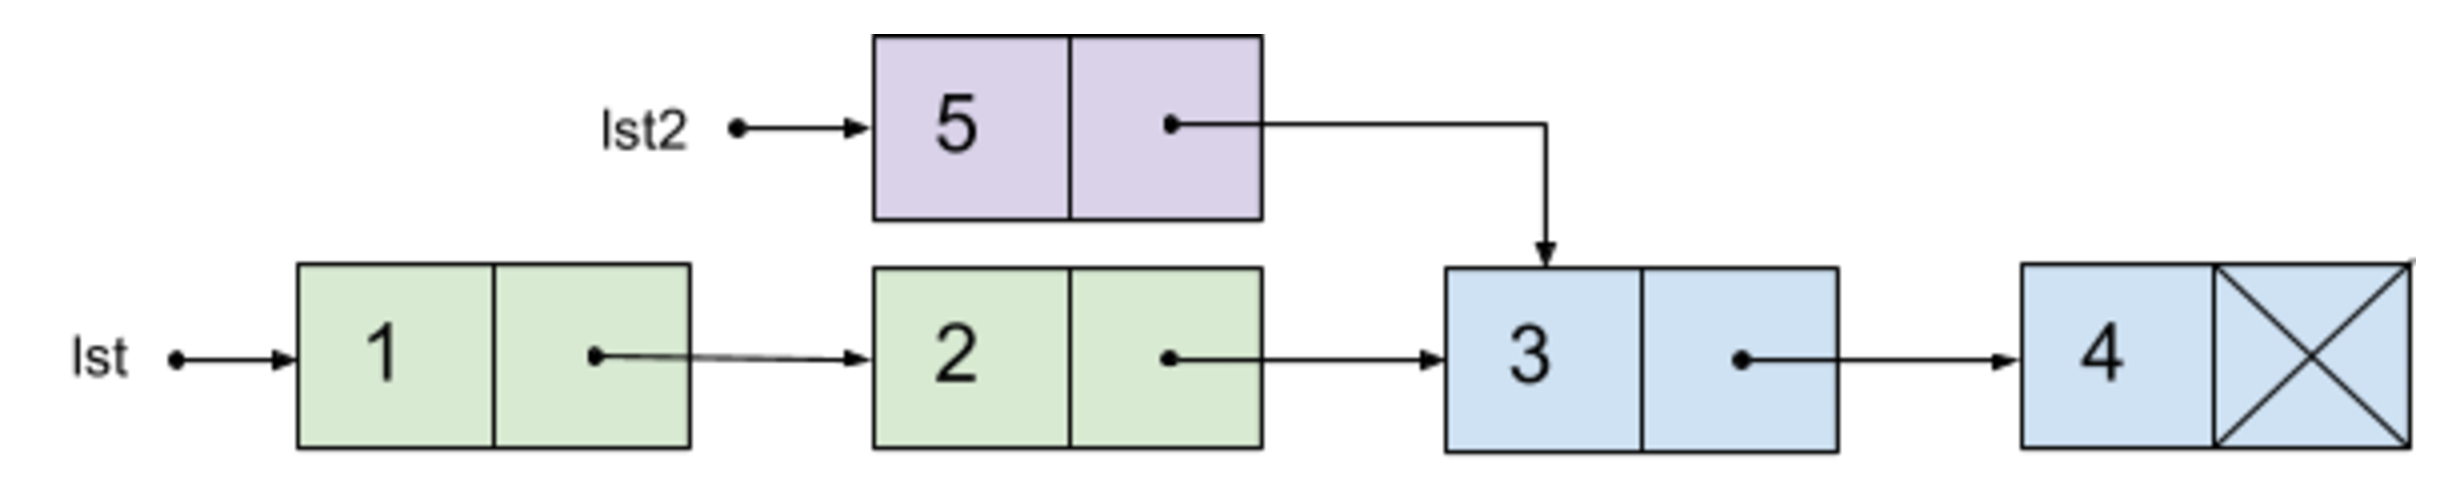
\includegraphics[width=0.9\textwidth]{list1234.png}

  \item Det er nemt at hægte et ekstra element på starten af en liste (\texttt{::}).

  \item Det er \textbf{IKKE} nemt (læs: hurtigt) at tilgå det sidste element i en liste.

  \item Lister er \emph{immutable}, dvs elementer kan ikke opdateres.

  \item Hvorfor kan immutabilitet være godt?
  \end{itemize}
\end{footnotesize}
\end{frame}

\begin{frame}[fragile]
\begin{footnotesize}
  \head{Repræsentationen af arrays}

  \begin{itemize}
  \item Syntax:
\begin{lstlisting}[numbers=none,frame=none]
let arr = [|1;2;3;4|]
\end{lstlisting}

  \item Lagerrepræsentation: \\
    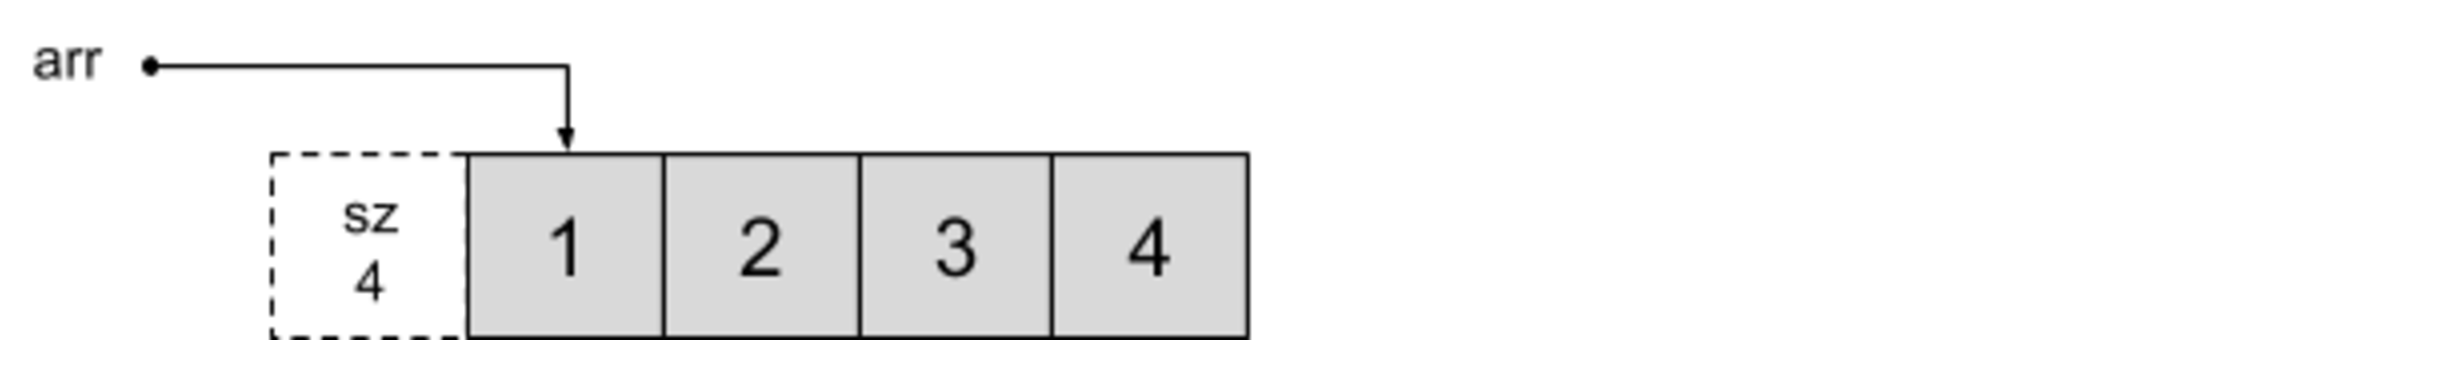
\includegraphics[width=0.9\textwidth]{array1234.png}
  \item Det er \textbf{IKKE} nemt at tilføje ekstra elementer.
  \item Det er nemt (hurtigt) at læse ethvert element i et array.

  \item Arrays er \emph{mutable}, dvs det er muligt (hurtigt) at
    opdatere ethvert element.
  \end{itemize}
\end{footnotesize}
\end{frame}

\subsection*{Konklusion}
\begin{frame}[fragile]
  \headsp{Konklusion}

  \vspace{3mm}
  \tableofcontents
\end{frame}

\end{document}
